% mẫu latex dùng cho đồ án 1, đồ án 2, và luận văn tốt nghiệp
% trường đại học sư phạm kỹ thuật tp hcm
% khoa điện điện tử
% bộ môn máy tính - viễn thông
% template được xây dựng lại dựa trên https://github.com/thanhhungqb/thesis-template
% mọi thắc mắc liên hệ: TS. Huỳnh Thế Thiện
\documentclass[a4paper, oneside]{book}
\usepackage[fontsize=14pt]{scrextend}
\usepackage{setspace}
\usepackage[utf8]{inputenc} 
\usepackage[T1]{fontenc} 
\usepackage[vietnamese,english]{babel} 

\usepackage[
singlelinecheck=false % <-- important
]{caption}
\usepackage{cite}
\usepackage{amsmath,amssymb,amsfonts}
\usepackage{algorithmic}
\usepackage{graphicx}
\usepackage{textcomp}
\usepackage{epsfig}
\usepackage{multirow}
\usepackage{xcolor}
\usepackage{float}
\usepackage{subfigure}
\usepackage[hidelinks]{hyperref}
\usepackage{mathptmx}
\usepackage{fancyhdr}
\usepackage{algorithm2e}
\usepackage{hmcutethesis}
\usepackage{indentfirst}


% {\fontsize{20}{1}\selectfont \textbf{\parbox[c][3cm]{0.9\linewidth}{ \centering \@tname }}} \\[1cm]

\ctname{\textbf{KỸ THUẬT NHẬN DIỆN PHỔ TÍN HIỆU CHO 5G VÀ LTE DỰA TRÊN CÁC PHƯƠNG PHÁP HỌC SÂU}} 
\cmjname{\textbf{NGÀNH KỸ THUẬT ĐIỆN TỬ}}

\cstuname{\textbf{Nguyễn Duy Huân} \\
[3pt] MSHV: 2390703} % với nhóm 1 sinh viên
\csSupervise{TS. \textbf{Huỳnh Thế Thiện}}
\cttime{08/2024}



\thesislayout
\setstretch{1.5}

\begin{document}
%-	Bìa cứng - màu xanh dương, chữ mạ vàng (xem mẫu đính kèm)
%-	Trang tên (tờ lót): chất liệu giấy, nội dung giống như bìa LV
%-	Ở gáy LV: in nhan đề LV (có thể in tóm tắt nếu nhan đề quá dài), size 15 – 17
%-	Phiếu Nhiệm vụ LV, chấm điểm Hướng dẫn & Phản biện (đã ký): nhận từ GVHD & GVPB sau khi bảo vệ (theo lịch hẹn).
%-	Lời cam đoan
%-	Lời cảm ơn/ Lời ngỏ
%-	Tóm tắt LV
%-	Mục lục
%-	Danh mục, bảng biểu, hình ảnh, ... (nếu có)
%-	Nội dung LV
%-	Danh mục TL tham khảo
%-	Phụ lục (nếu có)
\coverpage
\frontmatter

% Lý lịch khoa học ================================================
\begin{background}
\subsubsection*{Thông Tin Cá Nhân}

\begin{itemize}
    \footnotesize
    \item \textbf{Họ và Tên:} NGUYỄN DUY HUÂN
    \item \textbf{Ngày Sinh:} 29/30/2001
    \item \textbf{Địa chỉ:} Khối phố 1, An Sơn, Tam Kỳ, Quảng Nam
    \item \textbf{Email:} huan2931@gmail.com
    \item \textbf{Điện Thoại:} +84 8660 78421
\end{itemize}

\subsubsection*{Học Vấn}

\begin{itemize}
    \footnotesize
    \item \textbf{Bằng cấp cao nhất:} Kỹ sư
    \item \textbf{Nơi đào tạo:} Đại học Sư Phạm Kỹ Thuật thành phố Hồ Chí Minh
    \item \textbf{Chuyên ngành:} Kỹ thuật máy tính
    \item \textbf{Thời gian hoàn thành:} 2019-2023
\end{itemize}

\subsubsection*{Kinh Nghiệm Làm Việc}

\begin{itemize}
    \footnotesize
    \item \textbf{Tên công ty hoặc tổ chức:} Tập đoàn Công nghiệp – Viễn thông Quân đội (Viettel)
    \item \textbf{Chức vụ:} Nhân viên
    \item \textbf{Thời gian làm việc:} 05/2024 đến nay
\end{itemize}



\begin{table}[!h]
\centering
\begin{tabular}{p{3cm} p{3cm} p{3cm} p{3cm}}
&  & \multicolumn{2}{c}{Người khai thông tin} \\
&  & \multicolumn{2}{c}{\textit{(Ký và ghi rõ họ tên)}} \\
&  &             &            \\
&  &             &            \\
&  &             &            \\
&  &             &            \\
&  & \multicolumn{2}{c}{Nguyễn Duy Huân}
\end{tabular}
\end{table}
\end{background}

% lời cảm ơn ================================================
\begin{acknowledgments}

Trước tiên, xin được thể hiện lòng biết ơn sâu sắc đến TS. Huỳnh Thế Thiện, giảng viên tại trường đại học Sư Phạm Kỹ Thuật thành phố Hồ Chí Minh, vì những đề xuất và hỗ trợ quý báu của thầy đã giúp tôi có đủ điều kiện để thực hiện đề tài này. Hơn nữa, những kinh nghiệm và nghiên cứu khoa học của thầy trong lĩnh vực học máy và trí tuệ nhân tạo cung cấp cho tôi những ý tưởng và cơ hội để hoàn thành tốt đề tài này. Xin chân thành cảm ơn các quý thầy cô giảng viên tại trường đại học Sư Phạm Kỹ Thuật thành phố Hồ Chí Minh, đặc biệt là các thầy cô trong ngành kỹ thuật điện tử, khoa Điện - Điện Tử, đã giảng dạy và hỗ trợ tôi trong suốt quá trình học tập tại trường. Những đóng góp quý báu của các thầy cô đã góp phần quan trọng vào sự thành công của đề tài này.
\\
\begin{table}[!h]
\centering
\begin{tabular}{p{3cm} p{3cm} p{3cm} p{3cm}}
&  & \multicolumn{2}{c}{Người thực hiện luận văn} \\
&  & \multicolumn{2}{c}{\textit{(Ký và ghi rõ họ tên)}} \\
&  &             &            \\
&  &             &            \\
&  &             &            \\
&  &             &            \\
&  &             &            \\
&  &             &            \\
&  & \multicolumn{2}{c}{Nguyễn Duy Huân}
\end{tabular}
\end{table}
\end{acknowledgments}

% lời cam đoan ================================================
\begin{declaration}
	Người thực hiện đề tài cam đoan đề tài thực hiện dựa vào một số tài liệu trước đó và không sao chép nội dung, kết quả của các nghiên cứu trước đó. Các nội dung tham khảo đã được trích dẫn đầy đủ.
 \\
\begin{table}[!h]
\centering
\begin{tabular}{p{3cm} p{3cm} p{3cm} p{3cm}}
&  & \multicolumn{2}{c}{Người thực hiện luận văn} \\
&  & \multicolumn{2}{c}{\textit{(Ký và ghi rõ họ tên)}} \\
&  &             &            \\
&  &             &            \\
&  &             &            \\
&  &             &            \\
&  &             &            \\
&  &             &            \\
&  & \multicolumn{2}{c}{Nguyễn Duy Huân}    
\end{tabular}
\end{table}
\end{declaration}

% Tóm tắt LV ================================================
\begin{abstract}
     \noindent Trong lĩnh vực truyền thông không dây, việc cảm nhận phổ đóng một vai trò quan trọng trong việc phát triển các mạng khôn dây thế hệ mới, cho phép các thiết bị nhận diện và đáp ứng nhu cầu kết nối không dây. Trong nghiên cứu này, chúng tôi tập trung vào giải quyết những thách thức của cảm nhận phổ và giới thiệu một mô hình mạng sâu mới được đặt tên là SpecSenseNet, nhằm giải quyết vấn đề này trong việc cảm nhận thông tin truyền tải qua không khí. Mô hình của chúng tôi dựa trên kiến trúc của Unet nhưng tích hợp các kỹ thuật tiên tiến như depthwise separable convolution, recurrent residual block và Atrous Spatial Pyramid Pooling, nhằm giảm thiểu độ phức tạp của mạng mà vẫn duy trì hiệu suất dự đoán cao. Chúng tôi sử dụng một bộ dữ liệu tín hiệu tổng hợp gồm hai loại tín hiệu chính (5G new radio và LTE - long-term evolution) được điều chỉnh cho các mức độ nhiễu bổ sung khác nhau. 
 
%Kết quả mô phỏng cho thấy rằng mô hình của chúng tôi vượt trội với hiệu suất cảm nhận phổ xuất sắc, đồng thời giảm thiểu đáng kể độ phức tạp của mạng.
\end{abstract}	


% mục lục, danh sách bảng, danh sách hình tự động
\tableofcontents
\listoftables
\listoffigures


% danh sách các từ viết tắt =================================
\begin{abbreviation}
Dưới đây là danh mục các từ viết tắt được sử dụng trong luận văn.
\begin{table}[!h]
\renewcommand{\arraystretch}{1.3}
\begin{tabular}{p{3cm} p{11cm}}
\hline
\textbf{Các từ viết tắt} &  \textbf{Định nghĩa} \\
\hline
NR & new radio \\
LTE & long-term evolution \\
DL & deep learning \\
SpecSenNet & Spectrum Sensing Network \\
DSC & depthwise separable convolution \\
RRC & recurrent residual convolution \\
ASPP & Atrous Spatial Pyramid Pooling  \\
ML & machine learning \\
AI & Artificial Intelligence \\
CNN & convolutional neural network \\
FCN & fully connected network \\
RX & received signal \\
TX & transmitted signal \\
AWGN & Additive white Gaussian noise \\
STFT & short-time Fourier transform \\
SNR & signal-to-noise ratio \\
Deconv & Deconvolution \\
\hline
\end{tabular}
\end{table}
\end{abbreviation}	



\mainmatter


%  đánh số trang cho thesis ==================================
\fancypagestyle{plain}{
  \fancyhf{} % Clear header and footer
  \renewcommand{\headrulewidth}{0pt} % Remove header rule
  \fancyfoot[c]{\thepage} % Centered page number
}
\pagestyle{plain} % Apply the page style to all pages


% nội dung thesis được viết riêng cho từng chương (chapter)
\chapter{TỔNG QUAN}
\section{Giới thiệu}
Giới thiệu được viết tại đây ... 
\subsection{Giới thiệu về AI}
AI là ... 
\subsubsection{Giới thiệu về ML}
ML là machine learning~\cite{zhu2022}... 
\section{Mục tiêu}
Mục tiêu của đề tài ...

\section{Tình hình nghiên cứu}
Cách để trích dẫn bài báo xuất bản trong tạp chí~\cite{huynhthe2021}, bài báo được trình bài tại hội nghị~\cite{said2014biometric} và đường link của một trang web~~\cite{IoTDesignPro}

\section{Phương pháp nghiên cứu}
Để đạt được mục tiêu của đề tài, tôi sử dụng các phương pháp thu thập số liệu, thực nghiệm và phân tích tổng kết kinh nghiệm. 
\begin{itemize}
    \item Phương pháp thu thập số liệu:
    \begin{itemize}
        \item Sử dụng phương pháp quan sát: Tôi tiến hành quan sát trực ...
        \item Tiến hành cuộc phỏng vấn: Tôi tiến hành cuộc phỏng vấn ...
    \end{itemize}
    \item Phương pháp thực nghiệm: 
    \begin{itemize}
        \item Thiết kế và triển khai hệ thống: Tôi tiến hành thiết kế và triển khai ...
        \item Tiến hành thử nghiệm: Tôi thực hiện các bài kiểm tra và thử nghiệm hệ thống ...
    \end{itemize}    
    \item Phương pháp phân tích tổng kết kinh nghiệm: 
    \begin{itemize}
        \item Đánh giá hiệu quả: Tôi tiến hành đánh giá hiệu quả ...
        \item Phân tích dữ liệu: Tôi phân tích dữ liệu ...
        \item Tổng kết kinh nghiệm: Dựa trên kết quả phân tích, tôi tổng kết kinh nghiệm ...
    \end{itemize}
\end{itemize}

\section{Bố cục nội dung}
Báo cáo đồ án môn học 1 của tôi sẽ bao gồm 5 chương:
\begin{itemize}
    \item Chương 1: Tổng quan
    \item Chương 2: Cơ sở lý thuyết
    \item Chương 3: Thiết kế hệ thống
    \item Chương 4: Kết quả
    \item Chương 5: Kết luận và hướng phát triển.
\end{itemize}




% \begin{figure}[!t]
% 	\centering
% 	
\includegraphics[width=87.5mm]{hcmutelogo.png}
% 	\caption{SPWVD-TFIs of radar and communication waveform types.}
% 	\label{fig_example}
% \end{figure}

% \section{Yêu cầu và mục tiêu của đề tài}

% \subsection{Yêu cầu}

% Nghiên cứu thuật toán phân loại tin nhắn rác.

% Tạo ứng dụng chặn tin nhắn rác trên điện thoại thông minh (Android)

% \subsection{Mục tiêu}

% \subsubsection{Về kiến thức}

% Phân tích, giải quyết yêu cầu bài toán phân loại tin nhắn rác

% Nắm vững các thuật toán phân loại sử dụng

% Nắm các kỹ thuật xử lý văn bản: tách token, tính xác suất các token,\ldots

% Nắm các kiến thức lập trình di động (Android)

% \subsubsection{Về sản phẩm}

% \begin{table}[!t]
% \footnotesize
% \caption{Summary of Performance Comparison.}
% \begin{tabular}{@{}l r r r@{}}
% \hline
% \multirow{1}{*}{Networks}	& Size (params.) & Speed (ms) & Acc. ($\%$)  \\ \hline
% Lin~\textit{et al.}~\cite{lin2020unknown}	&$	1.4\mathrm{M}	$&$	0.0390	$&$	87.66	$\\
% Shen~\textit{et al.}~\cite{shen2022radar}	&$	6.1\mathrm{M}	$&$	0.0384	$&$	87.62	$\\
% % Huynh-The~\textit{et al.}~\cite{huynhthe2022racomnet}	&$	315\mathrm{K}	$&$	0.0536	$&$	89.91	$\\
% Huynh-The~\textit{et al.}~\cite{huynhthe2022racomnet}	&$	315\mathrm{K}	$&$	0.0586	$&$	89.91	$\\
% MobileNetv2~\cite{sandler2018mobilenetv2}	&$	2.2\mathrm{M}	$&$	0.0621	$&$	87.92	$\\
% ResNet50~\cite{he2016deep}	&$	23.5\mathrm{M}	$&$	0.0683	$&$	87.34	$\\
% Inception-V3~\cite{szegedy2016inception}	&$	21.8\mathrm{M}	$&$	0.1059	$&$	89.94	$\\
% EfficientNetb0~\cite{tan2019efficientnet}	&$	4.0\mathrm{M}	$&$	0.0823	$&$	89.47	$\\ 
% Sim-RadComNet	&$	180\mathrm{K}		$&$	0.1055	$&$	87.46	$\\
% Reg-RadComNet	&$	6.1\mathrm{M}		$&$	0.1270	$&$	89.47	$\\ \hline
% RadComNet ($2$ RSA modules)	&$	102\mathrm{K}		$&$	0.0602	$&$	82.85	$\\
% RadComNet ($3$ RSA modules)	&$	140\mathrm{K}		$&$	0.0644	$&$	86.85	$\\
% RadComNet ($4$ RSA modules)	&$	178\mathrm{K}		$&$	0.0679	$&$	89.87	$\\
% RadComNet ($5$ RSA modules)	&$	216\mathrm{K}		$&$	0.0712	$&$	90.56	$\\
% RadComNet ($6$ RSA modules)	&$	254\mathrm{K}		$&$	0.0744	$&$	90.89	$\\
% \hline
% \end{tabular}
% \label{tab_compare}
% \end{table}

% Tối ưu hóa bộ lọc, ứng dụng

% Nắm được quy trình phát triển sản phẩm: phân tích - thiết kế - hiện thực - kiểm tra.

% Phát triển ứng dụng thực tế, hướng sử dụng, tương tác.

% \section{Bố cục của luận văn}




\chapter{CƠ SỞ LÝ THUYẾT}
\section{Bảng và hình}
\subsection{Bảng}
Cách trình bày bảng~\ref{tab01} ... 

\begin{table}[!h]
\footnotesize
\caption{Bảng so sánh hiệu năng.}
\begin{tabular}{@{}l r r r@{}}
\hline
\multirow{1}{*}{Networks}	& Size (params.) & Speed (ms) & Acc. ($\%$)  \\ \hline
Method 1 &$	1.4\mathrm{M}	$&$	0.0390	$&$	87.66	$\\
Method 2	&$	6.1\mathrm{M}	$&$	0.0384	$&$	87.62	$\\
Method 3 &$	315\mathrm{K}	$&$	0.0586	$&$	89.91	$\\
MobileNetv2&$	2.2\mathrm{M}	$&$	0.0621	$&$	87.92	$\\
ResNet50&$	23.5\mathrm{M}	$&$	0.0683	$&$	87.34	$\\
Inception-V3&$	21.8\mathrm{M}	$&$	0.1059	$&$	89.94	$\\
EfficientNetb0&$	4.0\mathrm{M}	$&$	0.0823	$&$	89.47	$\\ 
Sim-RadComNet	&$	180\mathrm{K}		$&$	0.1055	$&$	87.46	$\\
Reg-RadComNet	&$	6.1\mathrm{M}		$&$	0.1270	$&$	89.47	$\\ \hline
RadComNet ($2$ RSA modules)	&$	102\mathrm{K}		$&$	0.0602	$&$	82.85	$\\
RadComNet ($3$ RSA modules)	&$	140\mathrm{K}		$&$	0.0644	$&$	86.85	$\\
RadComNet ($4$ RSA modules)	&$	178\mathrm{K}		$&$	0.0679	$&$	89.87	$\\
RadComNet ($5$ RSA modules)	&$	216\mathrm{K}		$&$	0.0712	$&$	90.56	$\\
RadComNet ($6$ RSA modules)	&$	254\mathrm{K}		$&$	0.0744	$&$	90.89	$\\
\hline
\end{tabular}
\label{tab01}
\end{table}

\begin{table}[!h]
\caption{Bảng điểm sinh viên}
\begin{tabular}{llll}
\hline
\multicolumn{1}{c}{MSSV} & \multicolumn{1}{c}{Họ} & \multicolumn{1}{c}{Tên} & \multicolumn{1}{c}{Điểm} \\ \hline
                         &                        & A                       & \multirow{2}{*}{8}       \\
                         &                        & B                       &                          \\
                         &                        &                         &                         
\end{tabular}
\label{tab02}
\end{table}

\subsection{Hình}
Hình được trình bày và tham khảo đến hình~\ref{fig01}...

\begin{figure}[!t]
	\centering
	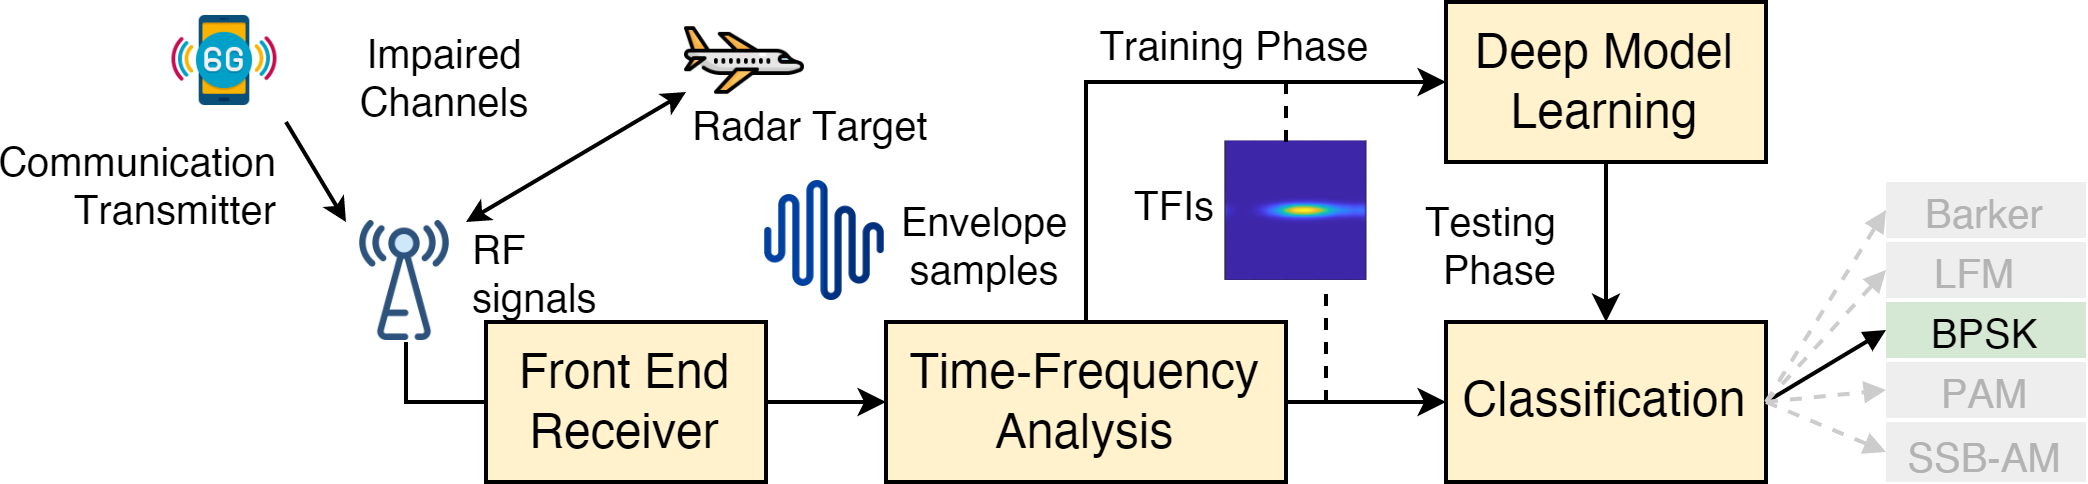
\includegraphics[width=14cm]{fig/fig01.png}    % hình được lưu trong thư mục fig (menu bên trái)
	\caption{Caption của hình là ...}
	\label{fig01}
\end{figure}

\subsubsection{Công thức toán học}
Công thức toán học được trình bày và đánh số tự động như trong công thức~(\ref{eqn01})...
\begin{equation}
h\left ( z \right )=\begin{cases}
z & \text{ if } z\geq 0 \\ 
0 & \text{ if } z < 0
\end{cases}.
\label{eqn01}
\end{equation}

\section{Cơ sở dữ liệu}
\subsection{Firebase Realtime Database}
Firebase Realtime Database ...
\subsubsection{Firebase A}
Firebase A là gì ...
\subsubsection{Firebase B}
Firebase B là gì ...
\subsection{Google Sheet}
Google Sheet là gì ...


\chapter{GIỚI THIỆU MẠNG HỌC SÂU ỨNG DỤNG TRONG PHÂN VÙNG ẢNH}
\section{Giới thiệu về mạng học sâu U-net}

\begin{figure}[h]
	\centering
	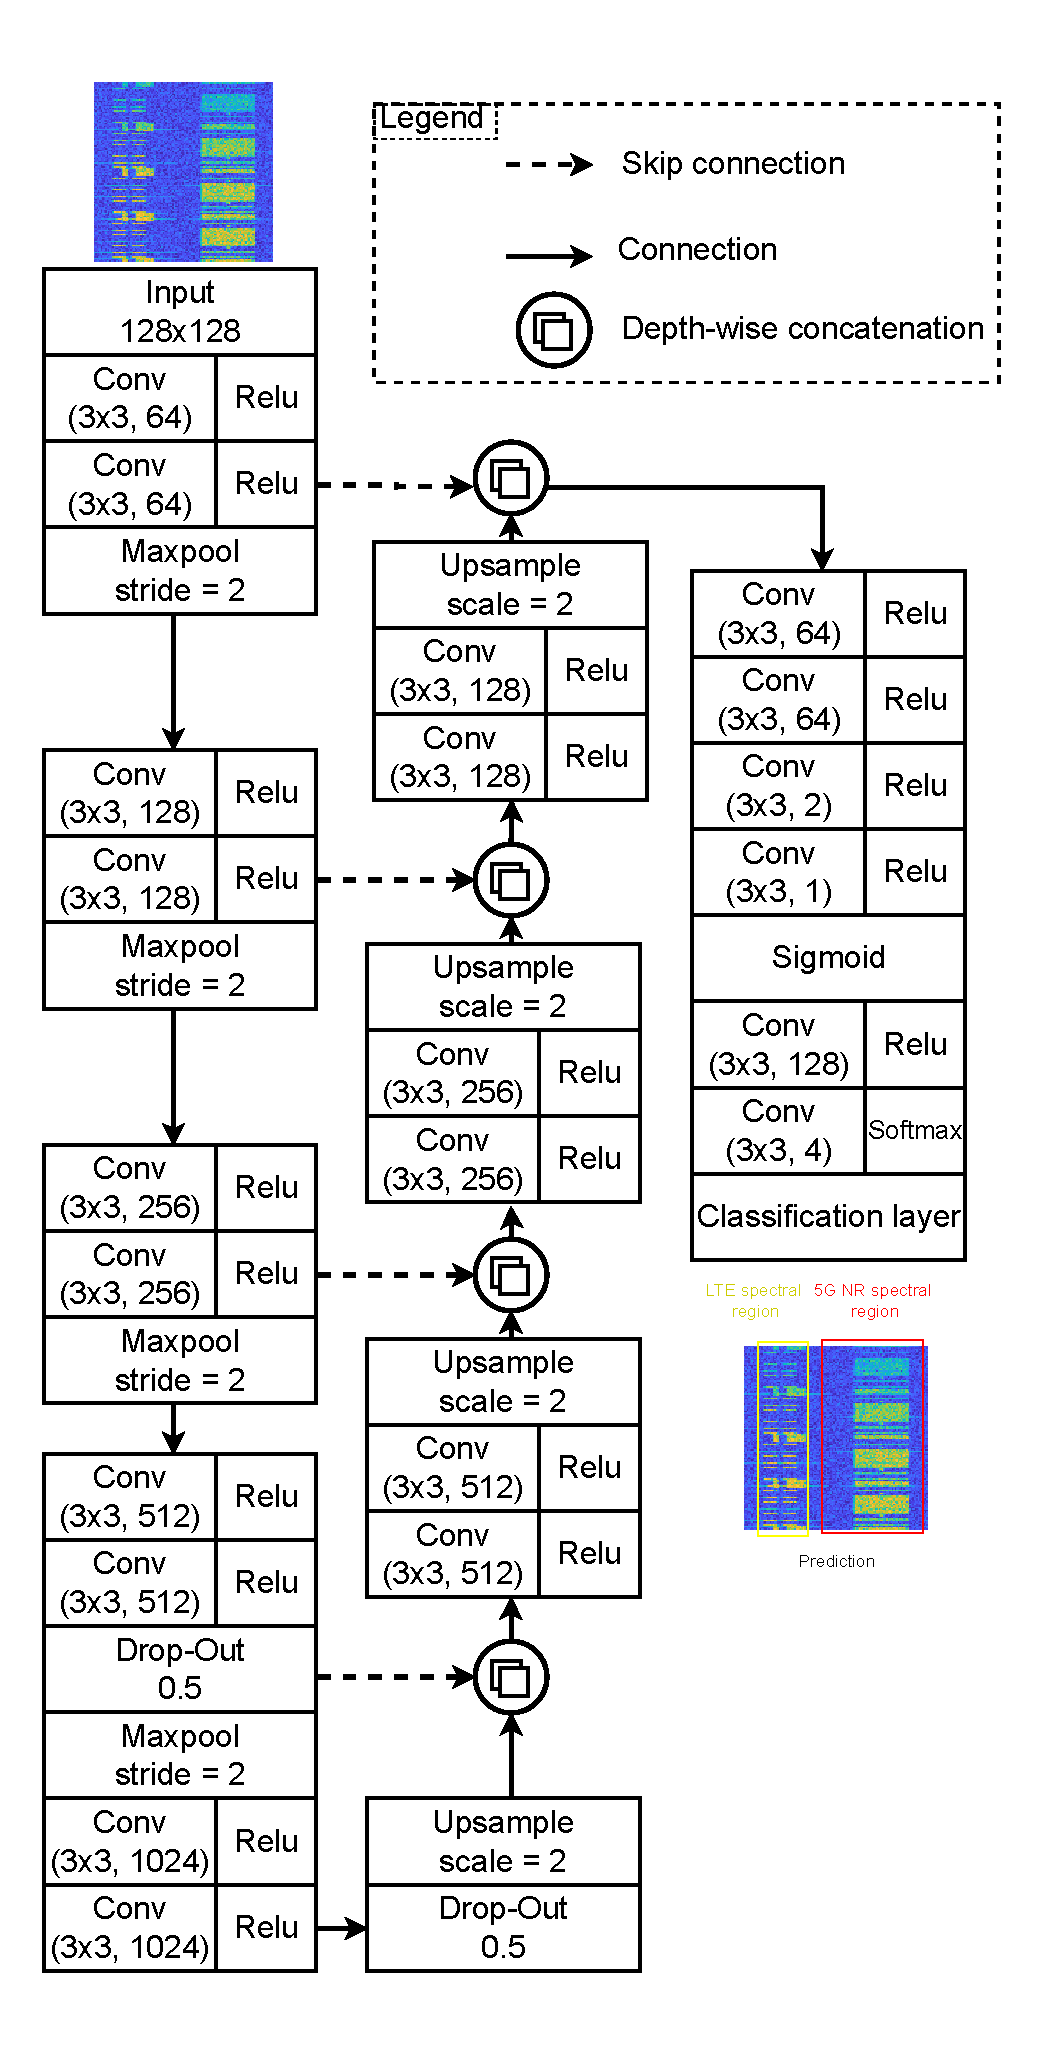
\includegraphics[width=80mm]{fig/Design-Unet.pdf}
        \captionsetup{justification=centering}
	\caption{Kiến trúc mạng U-net.}
	\label{fig_U-net}
\end{figure}

Mô hình mạng U-net được giới thiệu bởi tác giả Ronneberger \cite{aghalari2021brain} cùng với các cộng sự nhằm ứng dụng vào lĩnh vực nhận diện và phân loại ảnh chụp quang học. U-net là một mô hình mạng nơ-ron tích chập toàn phần đã được cải tiến và phát triển dựa trên cấu trúc của mạng tích chập truyền thống. Đặc trưng của U-net là cấu trúc đối xứng hình chữ "U", được minh họa ở Hình \ref{fig_U-net}. Phần mã hóa của mạng U-net tương tự như các mạng tích chập khác, bao gồm các lớp tích chập và tổng hợp tối đa để trích xuất đặc trưng từ ảnh. Trong Hình \ref{fig_U-net}, các lớp tích chập sử dụng cửa sổ trượt kích thước $3\times3$, và các lớp tổng hợp tối đa sử dụng cửa sổ trượt kích thước $2\times2$, giảm kích thước đầu vào đi một nửa cả về chiều dài và chiều rộng.

Thông qua các lần lặp của tích chập và tổng hợp tối đa, kích thước của ảnh sẽ giảm dần, tăng cường sự phức tạp của các đặc trưng được học. Để đảm bảo rằng thông tin chiều sâu đủ đáng kể, việc tăng số lớp tích chập ở cuối phần mã hóa là rất quan trọng để cải thiện hiệu suất học.

Một điểm đặc biệt của U-net là cấu trúc đối xứng của phần mã hóa và giải mã. Trong phần giải mã, việc mở rộng kích thước của ảnh tương đương với việc giảm kích thước của ảnh trong phần mã hóa tương ứng. Ngoài việc mở rộng kích thước, các lớp trong phần giải mã còn được kết nối đối xứng với các lớp tương ứng trong phần mã hóa, giúp khôi phục lại thông tin bị mất trong quá trình tổng hợp. Sau mỗi lần mở rộng trong phần giải mã, kết quả được kết hợp với kết quả của lớp giảm kích thước tương ứng trong phần mã hóa, trước khi đi qua các lớp tích chập và tiếp tục quá trình mở rộng.

\section{Mô hình mạng SegNet}

\begin{figure}[h]
	\centering
	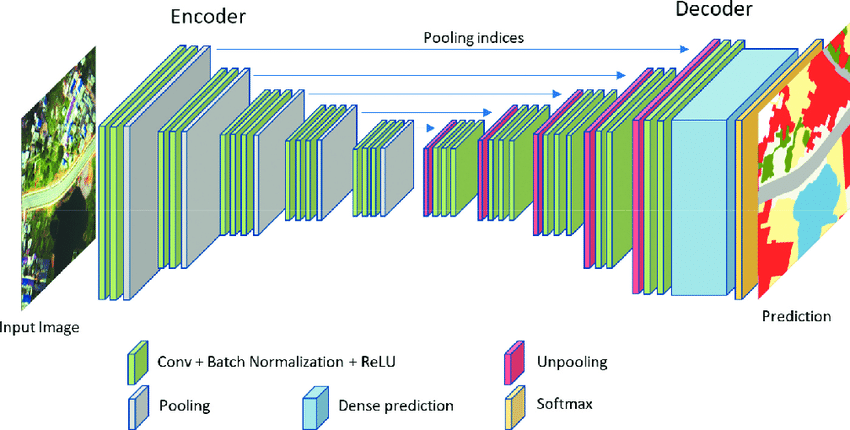
\includegraphics[width=120mm]{fig/SegNet-architecture.png}
        \captionsetup{justification=centering}
	\caption{Kiến trúc mạng SegNet (nguồn Internet).}
	\label{fig_SegNet}
\end{figure}

SegNet là một mô hình mạng nơ-ron tích chập được công bố bởi tác giả Badrinarayanan và các cộng sự~\cite{badrinarayanan2017segnet}, đặc biệt được thiết kế để giải quyết bài toán phân đoạn ảnh. Mô hình này có nhiều điểm tương đồng với U-net, bao gồm một phần mã hóa được xây dựng theo kiến trúc mạng tích chập thông thường, với các lớp tích chập và tổng hợp được lấy cảm hứng từ các mô hình nổi tiếng như VGG16, VGG19 và ResNet. Tuy nhiên, SegNet loại bỏ lớp kết nối đầy đủ ở cuối của mạng.

Như được minh họa trong Hình \ref{fig_SegNet}, phần mã hóa của SegNet sử dụng cấu trúc của mạng VGG16, bao gồm 13 lớp tích chập và 5 lớp giảm kích thước. Phần giải mã của SegNet cũng bao gồm các lớp mở rộng và tích chập, nhưng điểm đặc biệt và làm nên hiệu quả của mô hình nằm ở các lớp mở rộng.

Trong SegNet, đầu ra của các lớp mở rộng được mở rộng dựa trên vị trí ban đầu của các pixel tương ứng ở các lớp giảm kích thước trước đó. Để thực hiện điều này, vị trí của các pixel lớn nhất ở đầu vào của các lớp giảm kích thước được lưu giữ lại. Khi đi qua các lớp tích chập, các pixel đầu ra của lớp giảm kích thước sẽ được đưa về vị trí ban đầu của chúng trước khi thực hiện giảm kích thước.

So với U-net, SegNet không có các kết nối với các biểu đồ đặc trưng của các lớp trước, nhưng thay vào đó, thông tin quan trọng được lưu trữ và chuyển tiếp tới các lớp sau là vị trí của các pixel. Điều này làm cho SegNet tiêu tốn ít bộ nhớ hơn trong các ứng dụng và thiết bị nhúng. Với phần giải mã phức tạp và lớn với nhiều tầng tích chập, SegNet đã cho thấy kết quả khả quan trong nhiều thử nghiệm thực tế.

\section{Mô hình mạng SqueezeSegV2}

\begin{figure}[h]
	\centering
	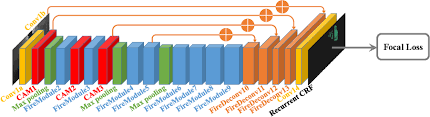
\includegraphics[width=120mm]{fig/SegNetV2-architecture.png}
        \captionsetup{justification=centering}
	\caption{Kiến trúc mạng SqueezeSegV2 (nguồn Internet).}
	\label{fig_SegNet}
\end{figure}

SqueezeSegV2~\cite{wu2019squeezesegv2}, là một mạng nơ-ron tích chập được phát triển dựa trên mô hình giải mã - mã hóa, đặc biệt thiết kế để phân loại dữ liệu điểm thu thập từ LiDAR trong ứng dụng phân vùng ngữ nghĩa. Đây là phiên bản nâng cấp của mô hình gốc có tên là SqueezeSeg. SqueezeSeg được tạo ra để phát hiện và phân loại các đối tượng quan trọng trong không gian 3D bằng cách biểu diễn phân vùng ngữ nghĩa 3D dưới dạng phân loại cho từng điểm dữ liệu. Dữ liệu điểm từ LiDAR được chuyển đổi thành hình ảnh 2D thông qua cơ chế phóng chiếu hình cầu, tạo nên một sự cân đối giữa độ chính xác và độ phức tạp.

Kiến trúc của SqueezeSeg được xây dựng bằng cách sử dụng các mô-đun Fire và mô-đun Deconvolution (Deconv), nhằm khắc phục việc mất mát thông tin chi tiết ở mức thấp do các phép giảm kích thước dữ liệu. Đặc biệt, SqueezeSegV2 cải tiến bằng việc giới thiệu một mô-đun tổng hợp ngữ cảnh mới (CAM) để giảm thiểu tác động tiêu cực của nhiễu dropout trong dữ liệu LiDAR, cũng như sử dụng hàm mất mát trọng tâm (focal loss) thay thế cho hàm mất mát cross-entropy ban đầu. Hàm mất mát trọng tâm giải quyết vấn đề mất cân bằng lớp bằng cách nhấn mạnh các mẫu âm trong quá trình huấn luyện.

So với U-net, SqueezeSegV2 tập trung vào việc phân loại dữ liệu điểm từ LiDAR thay vì phân đoạn hình ảnh. Điều này làm cho SqueezeSegV2 phù hợp hơn trong các ứng dụng cụ thể như tự lái xe, nơi mà dữ liệu LiDAR là quan trọng. SqueezeSegV2 cũng có một kiến trúc mạng phức tạp và các cải tiến trong hàm mất mát, giúp cải thiện độ chính xác và hiệu suất của mô hình. Tuy nhiên, U-net vẫn được ưa chuộng trong các ứng dụng phân đoạn hình ảnh chung do tính linh hoạt và khả năng áp dụng rộng rãi của nó.

\section{Đánh giá ưu và nhược điểm}
U-Net, SegNet và SqueezeSegV2 là ba mô hình quan trọng trong lĩnh vực phân vùng ngữ nghĩa ảnh, mỗi một trong số chúng đều có những đặc điểm và ưu điểm riêng.

U-Net nổi tiếng với cấu trúc đối xứng hình chữ "U", giúp nó trích xuất và tái tạo các đặc trưng cục bộ và toàn cục từ ảnh. Kiến trúc của U-Net giúp nó phù hợp với các tác vụ phân đoạn hình ảnh và đã được chứng minh hiệu quả trong nhiều ứng dụng y tế và địa lý. Tuy nhiên, U-Net có thể gặp khó khăn trong việc xử lý các đối tượng lớn và trong môi trường có nhiều nhiễu.

SegNet, trên cơ sở của mô hình tích chập truyền thống như VGG16 hoặc VGG19, chú trọng vào việc tái tạo vị trí của các pixel thông qua các lớp mở rộng và tích chập. Điều này giúp giữ lại thông tin về vị trí, đặc biệt quan trọng trong các ứng dụng nhúng và y tế. SegNet cũng có khả năng xử lý tốt các đối tượng lớn và nhiều nhiễu hơn so với U-Net.

SqueezeSegV2 là một mô hình tập trung vào việc phân loại dữ liệu điểm từ LiDAR, thích hợp cho các ứng dụng tự lái xe. Với cải tiến trong kiến trúc mạng và hàm mất mát, SqueezeSegV2 giúp cải thiện độ chính xác và hiệu suất trong việc phân loại các đối tượng trong không gian 3D từ dữ liệu LiDAR.

\section{Tệp dữ liệu khảo sát}
\begin{figure}[!h]
    \centering
    \footnotesize
    \begin{tabular}{ccccccc}
        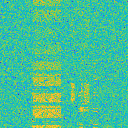
\includegraphics[width=0.12\textwidth]{fig/LTE_NR_0db.png} & 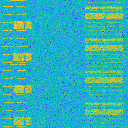
\includegraphics[width=0.12\textwidth]{fig/LTE_NR_5db.png} &
        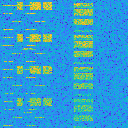
\includegraphics[width=0.12\textwidth]{fig/LTE_NR_10db.png}&
        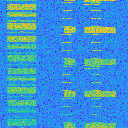
\includegraphics[width=0.12\textwidth]{fig/LTE_NR_15db.png}& 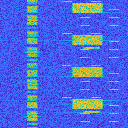
\includegraphics[width=0.12\textwidth]{fig/LTE_NR_20db.png}&
        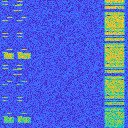
\includegraphics[width=0.12\textwidth]{fig/LTE_NR_25db.png}&
        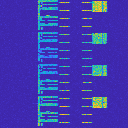
\includegraphics[width=0.12\textwidth]{fig/LTE_NR_30db.png}
        \\
        (a) & (b) & (c) & (d) & (e) & (f) & (g)
    \end{tabular}
    \caption{Dữ liệu giao thoa phổ 5G NR và LTE với SNR khác nhau: (a) 0 dB, (b) 5 dB, (c) 10 dB, (d) 15 dB, (e) 20 dB, (f) 25 dB, (g) 30 dB.}
    \label{fig_dataset5GLTE}
\end{figure}

\begin{figure}[!h]
    \centering
    \footnotesize
    \begin{tabular}{ccccccc}
        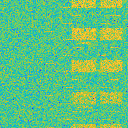
\includegraphics[width=0.12\textwidth]{fig/NR_frame_0db.png} & 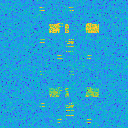
\includegraphics[width=0.12\textwidth]{fig/NR_frame_5db.png} &
        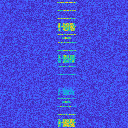
\includegraphics[width=0.12\textwidth]{fig/NR_frame_10db.png} &
        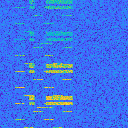
\includegraphics[width=0.12\textwidth]{fig/NR_frame_15db.png} & 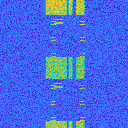
\includegraphics[width=0.12\textwidth]{fig/NR_frame_20db.png} &
        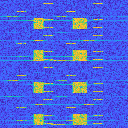
\includegraphics[width=0.12\textwidth]{fig/NR_frame_25db.png} &
        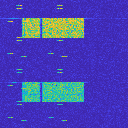
\includegraphics[width=0.12\textwidth]{fig/NR_frame_30db.png}
        \\
        (a) & (b) & (c) & (d) & (e) & (f) & (g)
    \end{tabular}
    \caption{Dữ liệu phổ 5G với SNR khác nhau: (a) 0 dB, (b) 5 dB, (c) 10 dB, (d) 15 dB, (e) 20 dB, (f) 25 dB, (g) 30 dB.}
    \label{fig_dataset5G}
\end{figure}

\begin{figure}[!h]
    \centering
    \footnotesize
    \begin{tabular}{ccccccc}
        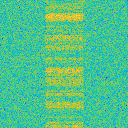
\includegraphics[width=0.12\textwidth]{fig/LTE_frame_0db.png} & 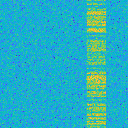
\includegraphics[width=0.12\textwidth]{fig/LTE_frame_5db.png} &
        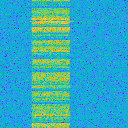
\includegraphics[width=0.12\textwidth]{fig/LTE_frame_10db.png} &
        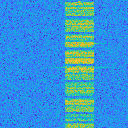
\includegraphics[width=0.12\textwidth]{fig/LTE_frame_15db.png} & 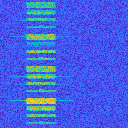
\includegraphics[width=0.12\textwidth]{fig/LTE_frame_20db.png} &
        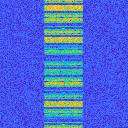
\includegraphics[width=0.12\textwidth]{fig/LTE_frame_25db.png} &
        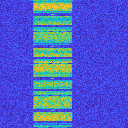
\includegraphics[width=0.12\textwidth]{fig/LTE_frame_30db.png}
        \\
        (a) & (b) & (c) & (d) & (e) & (f) & (g)
    \end{tabular}
    \caption{Dữ liệu phổ LTE với SNR khác nhau: (a) 0 dB, (b) 5 dB, (c) 10 dB, (d) 15 dB, (e) 20 dB, (f) 25 dB, (g) 30 dB.}
    \label{fig_datasetLTE}
\end{figure}

\begin{table}[h]
\centering
\caption{Thông tin về dữ liệu đầu vào cho mỗi phân loại}
\label{tab2}
\begin{tabular}{c|c|c|c}
\hline
\hline
\multicolumn{4}{c}{\textbf{Dataset Information}} \\
\hline
\textbf{Category} & \textbf{No.Samples} & \textbf{Image size} & \textbf{SNR (dB)}\\
\hline
\hline
LTE         & $5,000$ & $128 \times 128$ & $[0, 30]$ \\
5G          & $5,000$ & $128 \times 128$ & $[0, 30]$ \\
5G and LTE  & $5,000$ & $128 \times 128$ & $[0, 30]$ \\
\hline
\hline
\end{tabular}
\end{table}

Trong dự án nghiên cứu này, chúng tôi đã phải đối mặt với những thách thức thực tế, từ việc quản lý chi phí cho đến bảo vệ quyền riêng tư. Để nắm bắt bức tranh toàn diện về mạng 5G và LTE, chúng tôi đã sử dụng bộ công cụ 5G trong Matlab để tạo ra một tập dữ liệu phổ tổng hợp, bao gồm ba loại chính: 5G, LTE và các khung giao thoa giữa 5G và LTE.

Tập dữ liệu của chúng tôi bao gồm tổng cộng 5,000 mẫu cho mỗi loại, mỗi mẫu có kích thước hình ảnh là $128 \times 128$. Đặc biệt, chúng tôi đã khám phá một loạt các mức độ tín hiệu tạp âm-tỷ lệ tín hiệu (SNR) từ $0$ đến $30$ dB, để mô phỏng các tình huống khác nhau trong môi trường thực tế.


\section{Kết luận}
Trong đề tài này, học viên đã đề suất đề tài liên quan dến giám sát phổ tín hiệu dựa trên các mô hình học sâu, nhằm mục đích phát hiện các dải băng tần chưa được sử dụng và cấp phát cho các loại sóng di động cũng như ra-da khác. Dựa trên sự so sánh giữa các mô hình học sâu và những kinh nghiệm đã được tích lũy từ những đề tài nghiên cứu trước đó, học viên quyết định chọn mô hình U-net để tiếp tục tìm hiểu chi tiết và tìm ra giải pháp tăng cường hiệu năng của mô hình học sâu U-net sao cho đáp ứng được nhu cầu thực tế của đề tài. Việc lựa chọn U-Net cho việc cảm biến phổ có nhiều ưu điểm quan trọng:

\begin{itemize}
    \item \textbf{Xử lý hình ảnh 2D:} U-Net được thiết kế đặc biệt cho việc phân đoạn hình ảnh, phù hợp cho dữ liệu từ cảm biến phổ trong không gian 2D.
    \item \textbf{Kiến trúc đặc biệt:} Kiến trúc đối xứng hình chữ "U" của U-Net giúp nó trích xuất đặc trưng cục bộ và toàn cục từ ảnh một cách hiệu quả. Điều này rất hữu ích trong việc xử lý dữ liệu từ cảm biến phổ, nơi mà việc trích xuất các đặc trưng quan trọng từ dữ liệu là cần thiết.
    \item \textbf{Độ linh hoạt:} U-Net có thể dễ dàng được điều chỉnh và tinh chỉnh cho các yêu cầu cụ thể của ứng dụng cảm biến phổ. Cấu trúc mạng linh hoạt và khả năng đào tạo hiệu quả giúp nó thích hợp cho nhiều loại dữ liệu và nhiều tác vụ khác nhau.
    \item \textbf{Hiệu suất và hiệu quả:} U-Net đã được chứng minh hiệu quả trong nhiều ứng dụng phân đoạn hình ảnh, bao gồm cả việc xử lý dữ liệu từ cảm biến phổ. Với khả năng học và trích xuất đặc trưng tốt, U-Net có thể giúp tăng cường hiệu suất của hệ thống cảm biến phổ và giảm thiểu sai số.
    \item \textbf{Sử dụng trong các ứng dụng thực tế:} U-Net đã được sử dụng rộng rãi trong nhiều lĩnh vực, từ y tế đến xe tự lái và nông nghiệp. Sự phổ biến và khả năng thích nghi của nó làm cho U-Net trở thành một lựa chọn hợp lý cho việc xử lý dữ liệu từ cảm biến phổ trong các ứng dụng thực tế.
\end{itemize}




\chapter{KẾT LUẬN VÀ ĐỊNH HƯỚNG PHÁT TRIỂN CHO CHUYÊN ĐỀ 2}
\section{Kết Luận}
Trong quá trình nghiên cứu, học viên đã tiếp cận và hiểu biết sâu hơn về các mô hình mạng nơ-ron, đặc biệt là mạng nơ-ron tích chập và lý thuyết học sâu. Họ cũng đã tìm hiểu về bài toán phân vùng ảnh và cách áp dụng học sâu vào bài toán này. Dựa trên kiến thức thu thập được, học viên đã phát hiện ra rằng mô hình U-Net là sự lựa chọn tốt nhất cho dự án của mình.

U-Net đã chứng minh được hiệu quả và linh hoạt của mình trong việc phân vùng ảnh. So với SqueezeSegV2 và SegNet, U-Net có những ưu điểm nổi bật. Đặc biệt, U-Net có khả năng xử lý tốt các đối tượng nhỏ và linh hoạt trong việc điều chỉnh và tinh chỉnh cho các nhiệm vụ cụ thể. Mô hình này cũng không đối mặt với các hạn chế như SqueezeSegV2, như khả năng nhận diện các vật thể nhỏ và yêu cầu tài nguyên tính toán cao.

Do đó, việc sử dụng U-Net sẽ giúp học viên giải quyết các yêu cầu của dự án một cách hiệu quả và linh hoạt hơn, đồng thời cũng giảm thiểu được các hạn chế mà các mô hình khác như SqueezeSegV2 và SegNet đang đối mặt.

\section{Hướng phát triển}


Trong tương lai, việc nghiên cứu sâu hơn về việc tối ưu hóa cấu trúc mạng và các hàm mất mát có thể giúp cải thiện hiệu suất của mô hình U-Net. Các nghiên cứu này có thể tập trung vào việc tinh chỉnh kiến trúc mạng để tối ưu hóa việc trích xuất đặc trưng và dự đoán. Ngoài ra, cải tiến các hàm mất mát cũng có thể giúp tăng độ chính xác của mô hình và giảm thiểu thời gian dự đoán.

Thêm vào đó, việc thu thập một tập dữ liệu đa dạng hơn cũng là một phần quan trọng trong quá trình nghiên cứu. Dữ liệu này nên bao gồm các vị trí đối tượng lớn hơn và các trường hợp bổ sung của các lớp thiểu số, để mô hình có khả năng học được từ những trường hợp đa dạng và phong phú hơn.

Khám phá các độ phân giải dữ liệu khác nhau cũng là một hướng nghiên cứu tiềm năng. Việc này có thể giúp phát hiện và giải quyết các nhược điểm trong việc phân đoạn ảnh và cung cấp những hiểu biết có giá trị để cải thiện hiệu suất của mô hình U-Net trong các ứng dụng thực tế.

% tài liệu tham khảo theo chuẩn IEEE
% tài liệu tham khảo được khai báo trong file refs.bib
\bibliographystyle{IEEEtran} % ieeetr
\bibliography{refs}

\end{document}
